\subsection{Beneficios del algoritmo de ajuste propuesto}

Para analizar las ventajas del algoritmo de ajuste de pesos propuesto, se
obtiene un conjunto de parámetros DFTB utilizando pesos fijos e iguales para
todas las aleaciones. En otras palabras, se saltea el paso de optimización de los
coeficientes $\boldsymbol{\xi}$. Estos nuevos conjuntos se denotan por A$_0$ y
B$_0$. En la Figura \ref{fig:residuos}a se muestra el valor absoluto de los
residuos de las energías de formación de las estructuras cristalinas para ambos
conjuntos y se los compara con los obtenidos para los conjuntos A y B con
los pesos $\check{\boldsymbol{\xi}}$ optimizados. Aunque alguna aleación en
particular aumenta el residuo de su energía de formación luego de la
optimización de pesos por estequiometría, se confirma que este paso mejora
la tendencia general en las predicciones.

\begin{figure}[h]
	\centering
	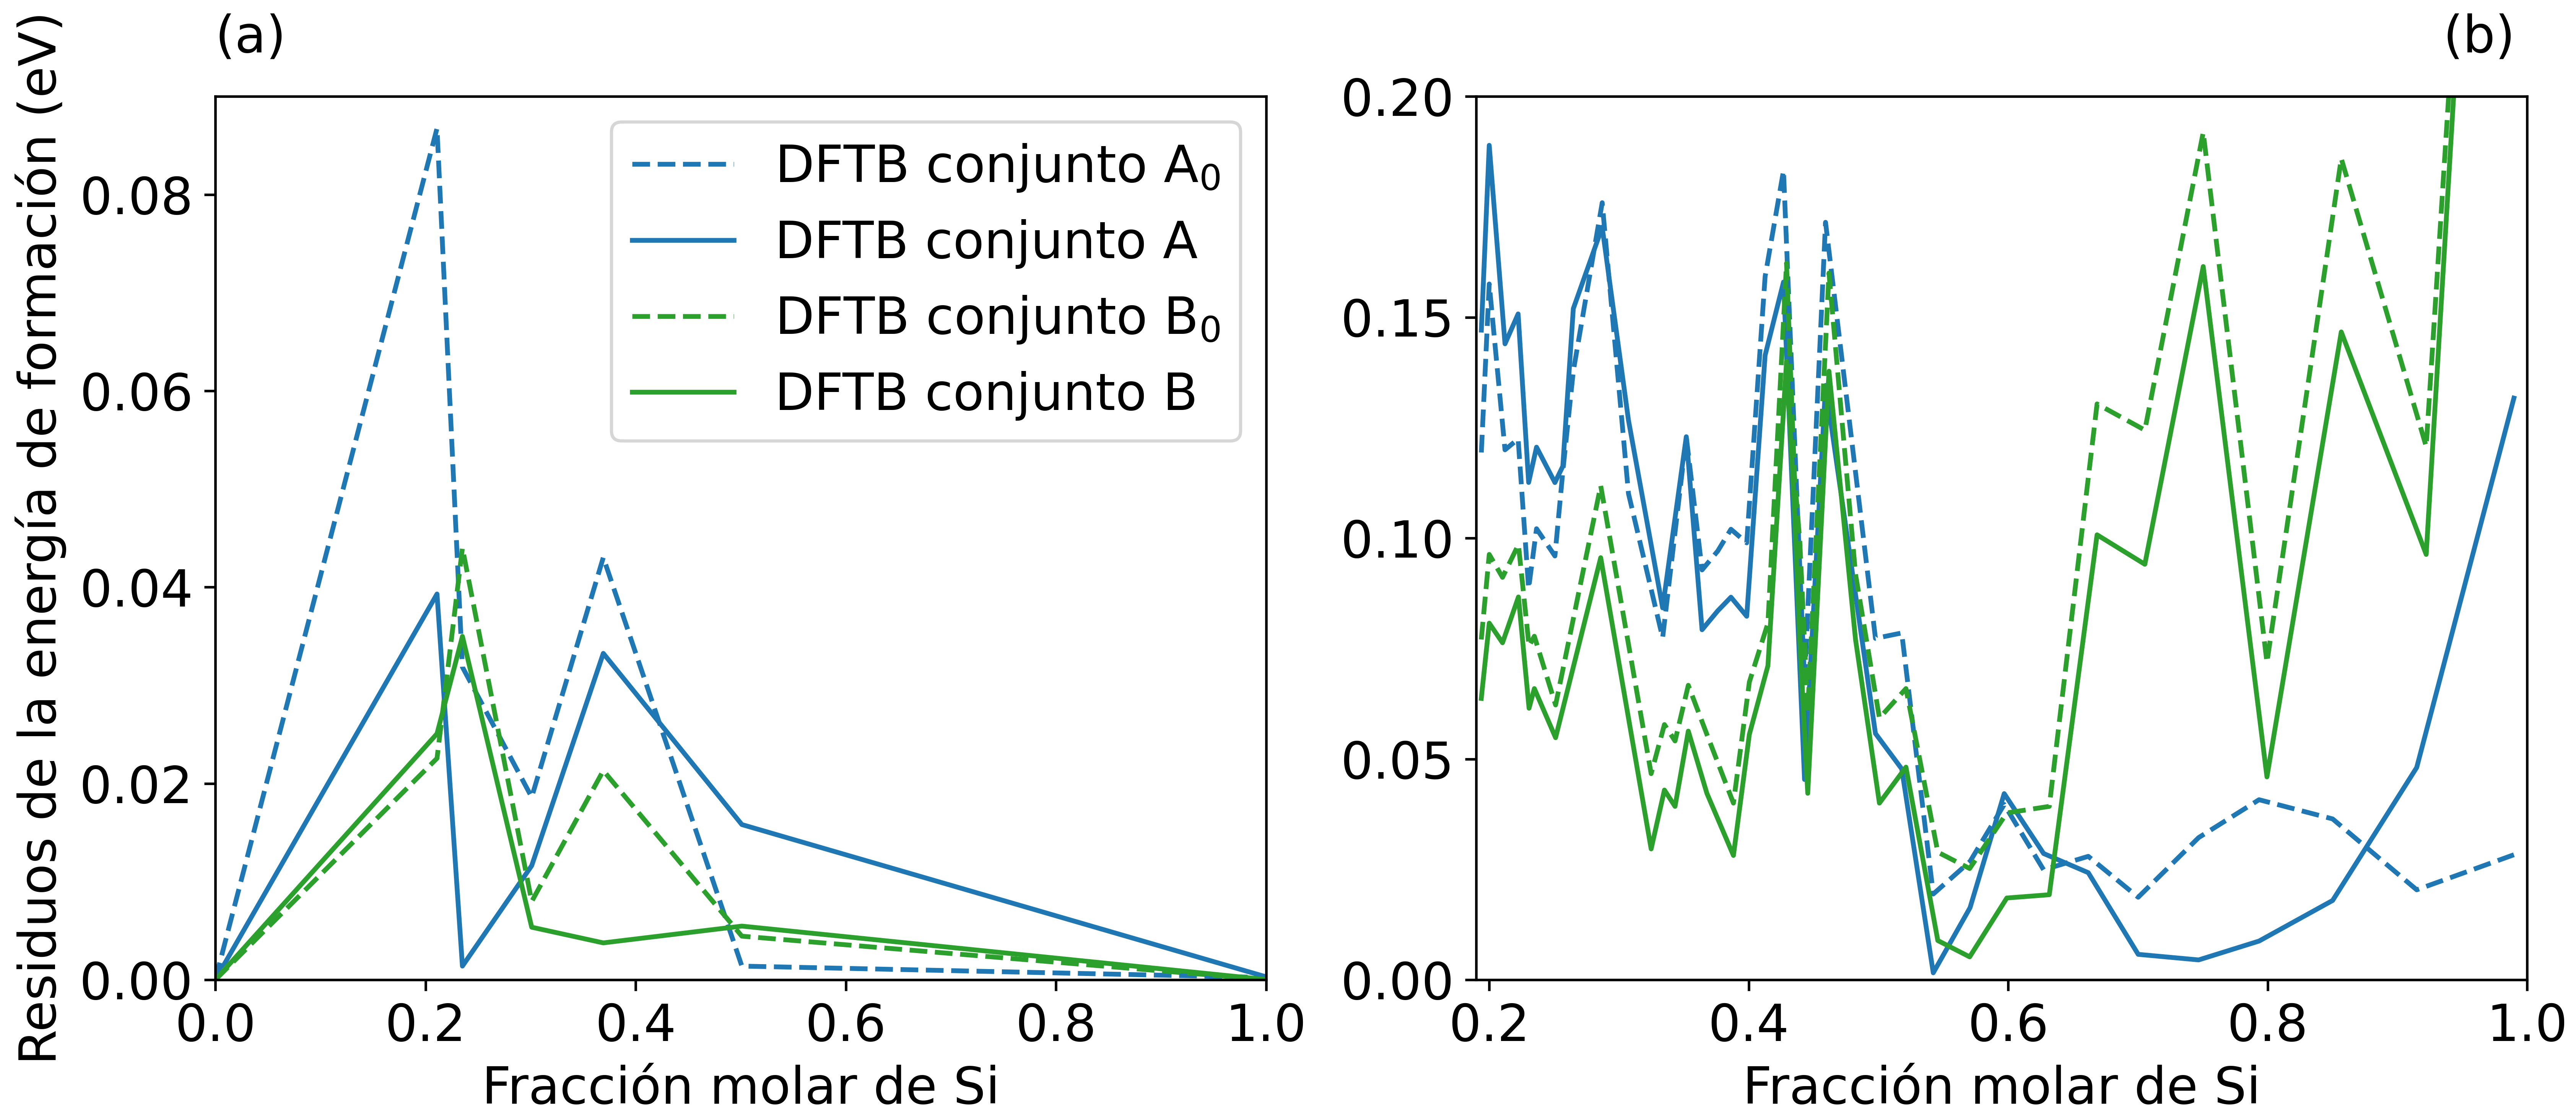
\includegraphics[width=\textwidth]{Silicio/modelo/resultados/residuos/residuos.png}
	\caption{Residuos de las energías de formación obtenidos con DFTB (respecto a
	DFT) con los conjuntos de parámetros antes de la optimización de los pesos
    $\boldsymbol{\xi}$ (A$_0$ y B$_0$) y después de la misma (A y B). (a) Estructuras 
    cristalinas de Li--Si de entrenamiento. (b) Estructuras amorfas de Li$_x$Si de
    evaluación.}
	\label{fig:residuos}
\end{figure}

Este chequeo también se realiza en el conjunto de evaluación de estructuras
amorfas en la Figura \ref{fig:residuos}b. De estos datos se concluye que el
algoritmo de ajuste propuesto en la sección \ref{s:algfit} ayuda a aumentar
la precisión a la hora de predecir las energías de formación. Esto es
especialmente cierto para el conjunto B, que para todas las aleaciones amorfas
presenta residuos menores que el conjunto B$_0$. En el caso del conjunto A, 
la optimización de pesos permite una mayor precisión entre $0.35 < \Theta < 0.9$ 
pero no para los valores extremos de $\Theta$. Esto puede deberse a que la 
optimización de pesos en este conjunto se focaliza en las aleaciones intermedias, 
mientras que los pesos de los elementos puros son considerablemente menores.
